% this TeX file provides an awesome example of how TeX will make super
% awesome tables, at the cost of your of what happens when you try to make a
% table that is very complicated.
% Originally turned in for Dr. Nico's Security Class
\documentclass[11pt]{article}


% Use wide margins, but not quite so wide as fullpage.sty
\marginparwidth 0.5in
\oddsidemargin 0.25in
\evensidemargin 0.25in
\marginparsep 0.25in
\topmargin 0.25in
\addtolength{\topmargin}{-.75in}
\textwidth 6in
\textheight 8.5in
% That's about enough definitions

\usepackage{fancyvrb,graphicx,float,indentfirst,tikz,circuitikz}
\usetikzlibrary{shapes.geometric, calc}
\tikzstyle{every node}=[trapezium left angle=60, trapezium right angle=120]
\usepackage{array}
\newcolumntype{C}[1]{>{\centering\let\newline\\\arraybackslash\hspace{0pt}}m{#1}}
\renewcommand{\arraystretch}{1.5}

\begin{document}

\author{
  Anderson, Anna\      \qquad\texttt{anna.anderson@colorado.edu}
  \and
  Cuthbertson, Sam\      \qquad\texttt{samuel.cuthbertson@colorado.edu}
  }

\title{Digital Logic: Project 2 Block Diagrams}
\maketitle

\begin{figure}[H]
    \centering
    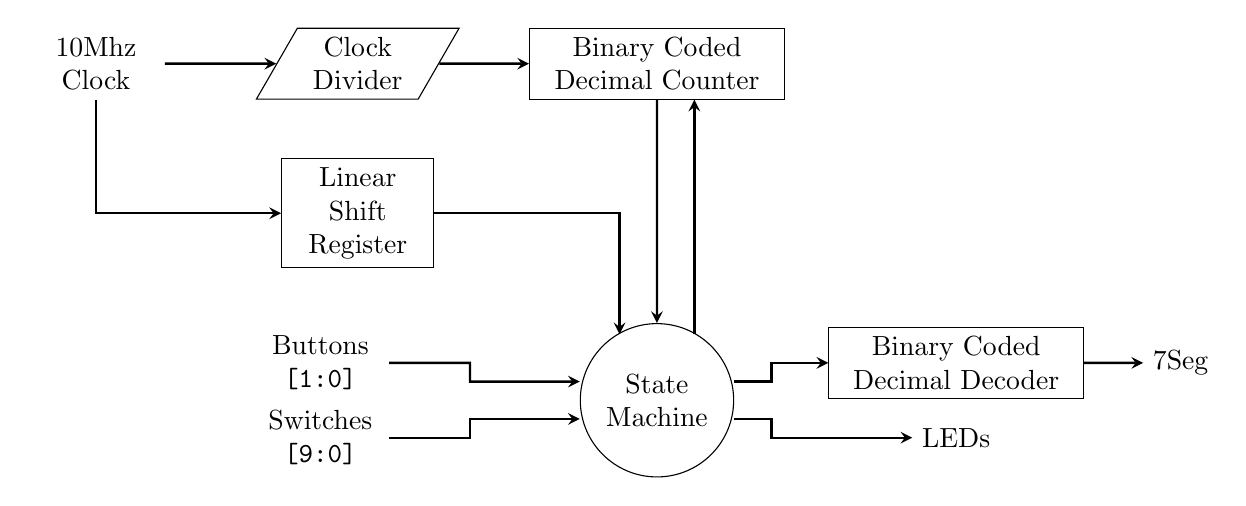
\begin{tikzpicture}[scale=0.95]

        \node[text width = 15mm, align=center] at (0,6) (ClkIn) {10Mhz Clock};
        \node[text width = 15mm, align=center] at (3,2) (Bin) {Buttons {\tt[1:0]}};
        \node[text width = 15mm, align=center] at (3,1) (Sin) {Switches {\tt[9:0]}};

        \node[rectangle, draw, text width=17mm, align=center] at (3.5,4) (LSR) {Linear Shift Register};
        \node[circle, draw, text width=15mm, align=center] at (7.5,1.5) (SM) {State Machine};
        \node[rectangle, draw, text width=30mm, align=center] at (7.5,6) (BCDC) {Binary Coded Decimal Counter};
        \node[trapezium, draw, text width=13mm, align=center] at (3.5,6) (ClkDiv) {Clock Divider};

        \node[rectangle, draw, text width=30mm, align=center] at (11.5,2) (BCDDC) {Binary Coded Decimal Decoder};
        \node at (14.5, 2) (7Seg) {7Seg};
        \node at (11.5, 1) (LEDs) {LEDs};

        \draw[->,>=stealth,line width=0.3mm] (ClkIn) -- (ClkDiv.west);
        \draw[->,>=stealth,line width=0.3mm] (Bin) -- ($(Bin)+(2,0)$) |- ($(SM.west)+(0,.25)$);
        \draw[->,>=stealth,line width=0.3mm] (Sin) -- ($(Sin)+(2,0)$) |- ($(SM.west)-(0,.25)$);
        \draw[->,>=stealth,line width=0.3mm] (ClkDiv) -- (BCDC);
        \draw[->,>=stealth,line width=0.3mm] (ClkIn) |- (LSR.west);
        \draw[->,>=stealth,line width=0.3mm] (LSR.east) -| ($(SM.north)-(.5,.15)$);
        \draw[->,>=stealth,line width=0.3mm] (BCDC.south) -- (SM);
        \draw[->,>=stealth,line width=0.3mm] ($(SM.north)+(.5,-.15)$) -- ($(BCDC.south)+(.5,0)$);
        \draw[->,>=stealth,line width=0.3mm] ($(SM.east)+(0,.25)$) -| ($(SM.east)+(.5,.25)$) |- (BCDDC.west);
        \draw[->,>=stealth,line width=0.3mm] ($(SM.east)-(0,.25)$) -| ($(SM.east)+(.5,-.25)$) |- (LEDs.west);
        \draw[->,>=stealth,line width=0.3mm] (BCDDC.east) -- (7Seg);

    \end{tikzpicture}
    \caption{Our block diagram for top.v.}
\end{figure}

\begin{figure}[H]
    \centering
    \begin{minipage}{0.5\textwidth}
        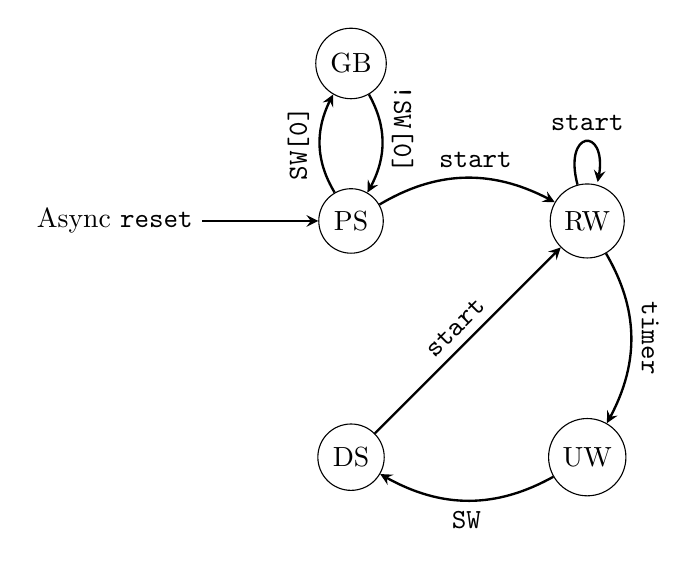
\begin{tikzpicture}[scale=1]

            \node at (0,6) (Reset) {Async {\tt reset}};
            \node[circle, draw] at (3,6) (Pause) {PS};
            \node[circle, draw] at (6,6) (RW) {RW};
            \node[circle, draw] at (6,3) (UW) {UW};
            \node[circle, draw] at (3,3) (DS) {DS};

            \node[circle, draw] at (3,8) (SkoBuffs) {GB};

            \draw[->,>=stealth,line width=0.3mm] (Reset) -- (Pause);
            \draw[->,>=stealth,line width=0.3mm] (DS) -- node[above, rotate=45] {\tt start} (RW);
            \draw[->,>=stealth,line width=0.3mm] (Pause) edge[bend left] node[above, pos=.55] {\tt start} (RW);
            \draw[->,>=stealth,line width=0.3mm] (RW) edge[loop above] node[above] {\tt start} (RW);
            \draw[->,>=stealth,line width=0.3mm] (RW) edge[bend left] node[above, rotate=270] {\tt timer} (UW);
            \draw[->,>=stealth,line width=0.3mm] (UW) edge[bend left] node[below] {\tt SW} (DS);

            \draw[->, >=stealth,line width=0.3mm] (Pause) edge[bend left] node[above, rotate=90] {\tt SW[0]} (SkoBuffs);\draw[->, >=stealth,line width=0.3mm] (SkoBuffs) edge[bend left] node[above, rotate=270, pos=.35] {\tt !SW[0]} (Pause);

        \end{tikzpicture}
    \end{minipage}
    \hfill
    \begin{minipage}{0.4\textwidth}
        \begin{tabular}{c|C{3.25cm} }
            State Name & Description \\
            \hline
            \hline
            PS & Mode we boot into, displays highscore. \\
            \hline
            GB & Diplays a scrolling ``Go Buffs''. \\
            \hline
            RW & Waits a random time interval. \\
            \hline
            UW & Counts the time spent here. \\
            \hline
            DS & Displays the value from the counter, updates highscore. \\

        \end{tabular}
    \end{minipage}
    \caption{Our graph for the State Machine in top.v, where {\tt B0} is the start button, {\tt B1} is the reset button, and {\tt SW} is assumed to be the correct switch. Additionally, all buttons are assumed to be active-low and all switches are assumed to be active-high.}
\end{figure}

\end{document}
